\section{Introduction}

\subsection[History of AI and ML]{History of \acl{AI} and \acl{ML}}

\begin{frame}
  \note{
    \begin{itemize}
    \item Present birth of AI: McCarthy, Dartmouth workshop, 1956
    \item Previous ideas
      \begin{itemize}
      \item Philosophy, logic, Turing machine, information theory, cybernetics
      \end{itemize}
    \item Birth of ML as a field of AI: Arthur Samuel, 1959
      \begin{itemize}
      \item Adaptation instead of explicit programming
      \end{itemize}
    \item Insist on broad approaches:
      \begin{itemize}
      \item symbolic \vs{} connexionist
      \item link with cognitive sciences
      \end{itemize}
    \item Concrete realizations:
      \begin{itemize}
      \item Modern programming languages: OO, more dynamic, CAS
      \item Problem solving: navigation on graphs
      \item Mc Carthy: as soon as it works, nobody calls it AI anymore
      \end{itemize}
    \item Over-optimistic preditions:
      \begin{itemize}
      \item Herbert Simon, 1958:  within ten years a digital computer will be
        the world's chess champiom
      \end{itemize}
    \end{itemize}
  }
  \frametitle{Birth \& early successes (1956--1973)}

  \begin{textblock}{100} (0,10)
    \begin{center}
      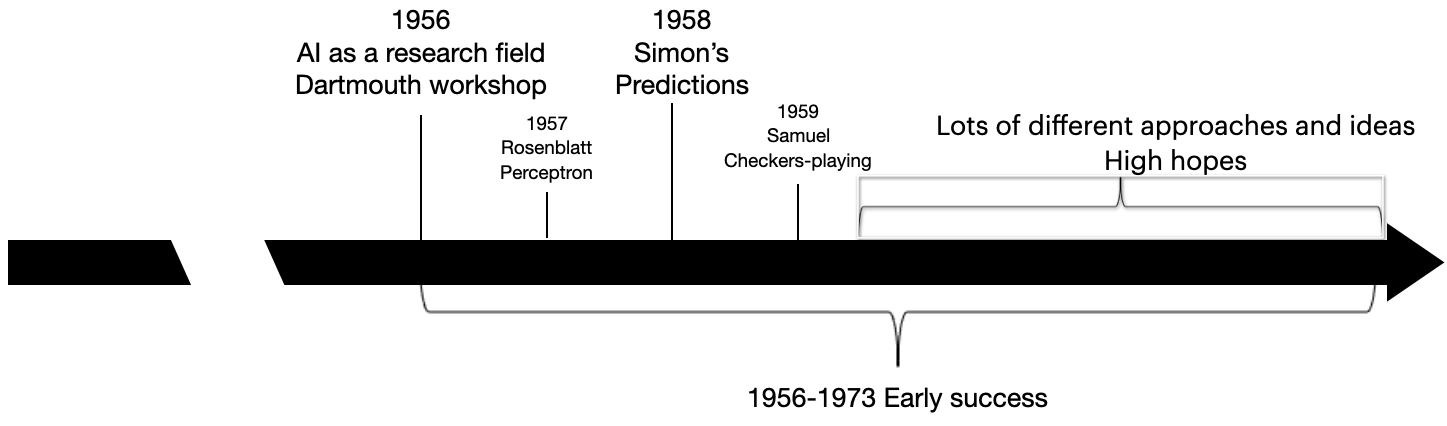
\includegraphics[width=0.95\textwidth]{img/ai_history_1956_1973.png}
    \end{center}
  \end{textblock}

  % Résumé de la frise
  \begin{textblock}{50}(0, 50)
    \begin{itemize}
      \item \aclu{AI} (1956)
        \begin{itemize}
        \item \footnotesize Discipline focused on creating systems capable of
          performing tasks that typically require human intelligence, such as
          problem-solving, decision-making, translation, \etc{}.
        \end{itemize}
      \item<2-> \acl{ML} (1959)
        \begin{itemize}
        \item \footnotesize Field of AI focused on the development and study of machines that can learn from data and generalize to unseen data.
        \end{itemize}
      \end{itemize}
    \end{textblock}

    % Résumé des réalisations
    \begin{textblock}{50}(50, 50)
      \begin{center}
        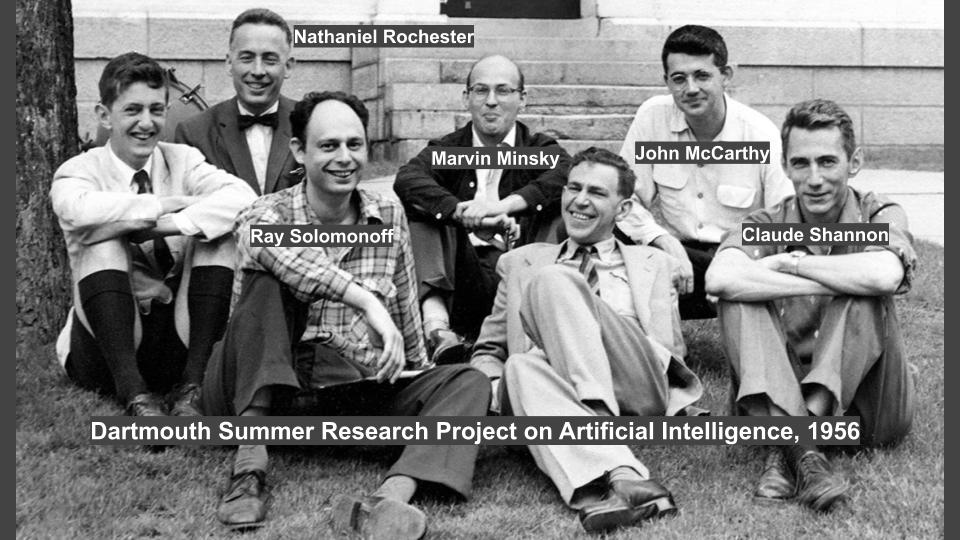
\includegraphics[width=0.9\textwidth]{img/dartmouth-conference.jpg}
      \end{center}
    \end{textblock}

\end{frame}


\begin{frame}
  \note{
    \begin{itemize}
    \item Second phase is made of so-called ``winters'' (periods of lower
      funding or... hype)
    \item However there was still lot of work
    \end{itemize}
  }
  \frametitle{AI winters and expert systems (1973-2000)}

  \begin{textblock}{100}(0,10)
    \begin{center}
      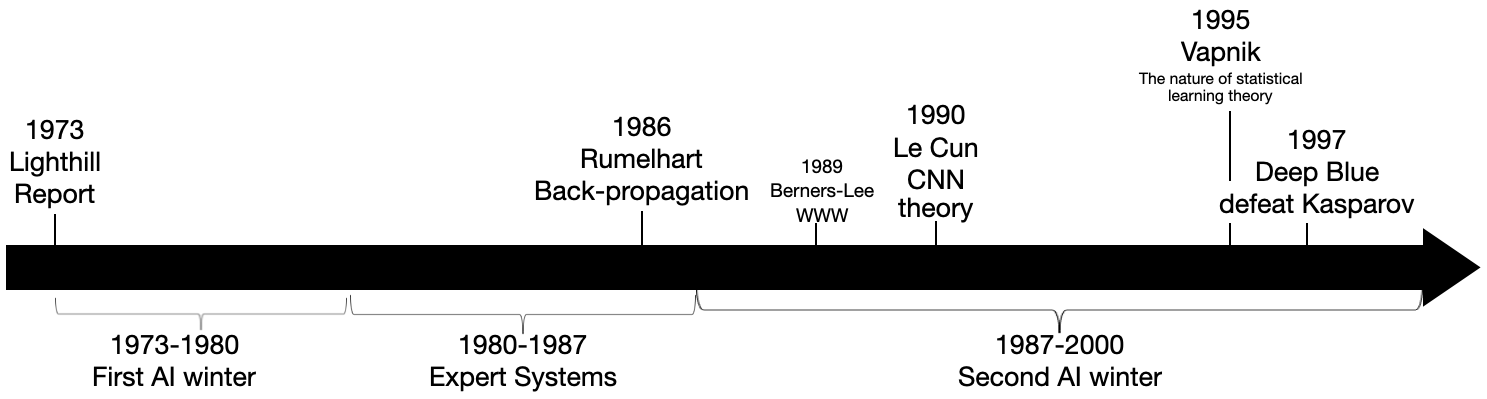
\includegraphics[width=0.95\textwidth]{img/ai_history_1973_2000.png}
    \end{center}
  \end{textblock}

  % Résumé de la frise
  \begin{textblock}{50}(0, 50)
    \begin{itemize}
    \item Lighthill report (1973):
      \begin{itemize}
      \item {\footnotesize ``In no part of the field have the discoveries made so far produced the major impact that was then promised''}
      \item Start of the First Winter
      \end{itemize}
    \item<2-> Proliferation of expert systems (1980s):
      \begin{itemize}
      \item Practical limitations
      \item Start of the Second Winter
      \end{itemize}
    \end{itemize}
  \end{textblock}

  % Enseignements, causes, etc.
  \begin{textblock}{50}(50, 50)
    \begin{itemize}
      \item<3-> Interesting work in the era:
      \begin{itemize}
      \item Technological development: WWW, Python, computing power
      \item Methodological development: statistical learning theory
      \item Deep Blue \vs{} Kasparov
      \item Premise of deep learning
      \end{itemize}
    \end{itemize}
  \end{textblock}

\end{frame}


\begin{frame}
  \note{
    \begin{itemize}
    \item Rise of learning due to work of previous period
    \item Rise of deep learning since 2012
    \item Importance of the amount of data
    \item Less theory
    \end{itemize}
  }
  \frametitle{Rise of Machine Learning and Deep Learning (2000-2024)}

  \begin{textblock}{100}(0,10)
    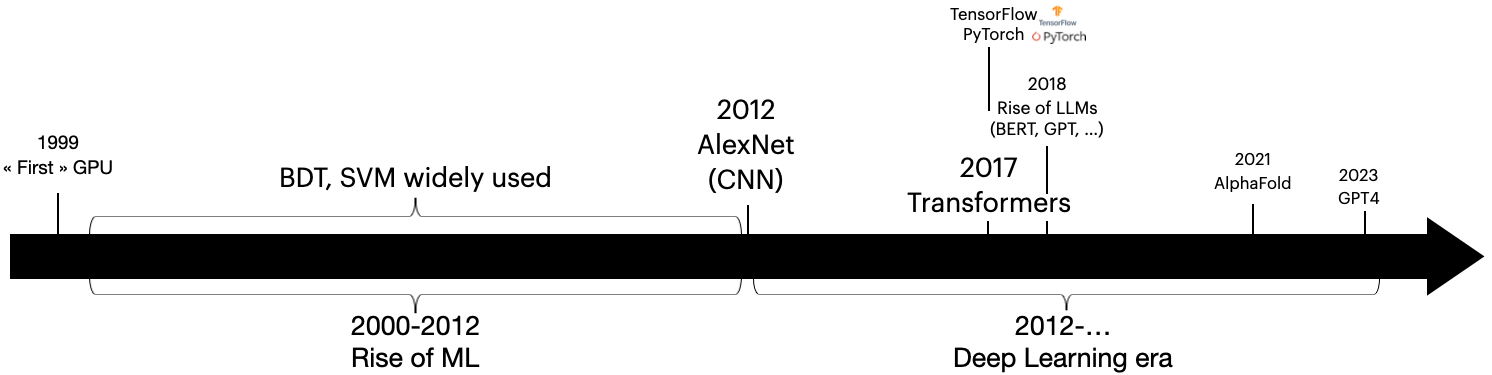
\includegraphics[width=\textwidth]{img/ai_history_2000_2024.png}
  \end{textblock}

  % Commentaire de la frise
  \begin{textblock}{50}(0, 50)
    \begin{itemize}
    \item Rise of \ac{ML} in the early 2000s
    \item<2-> Deep learning era:
      \begin{itemize}
      \item CNN: AlexNet (2012)
      \item Transformers (2017) leads to first LLMs (2018)
      \end{itemize}
    \end{itemize}
  \end{textblock}

  % Enseignements, causes, etc.
  \begin{textblock}{50}(50, 50)
    \onslide<3->{
      \begin{itemize}
      \item Neural networks are mature
      \item Practical causes:
        \begin{itemize}
        \item Lots of data
        \item Processing power (GPU) and storage capability
        \item Mature technology (langages, frameworks)
        \end{itemize}
      \end{itemize}
    }
  \end{textblock}

\end{frame}


\subsection{A word on data}

% Copied from FIDLE lesson 2
\begin{frame}
  \note{
    \begin{itemize}
    \item Modern data are of many different types
      \begin{itemize}
      \item Some tasks can only be applied to some type
      \item Some algorithms/methods are specific to some type
      \end{itemize}
    \item Numerical representation
    \end{itemize}
  }
  \frametitle{Types of data}

  \begin{textblock}{90}(5, 10)
    The world is made of different types of data (picture from FIDLE):
    \begin{center}
      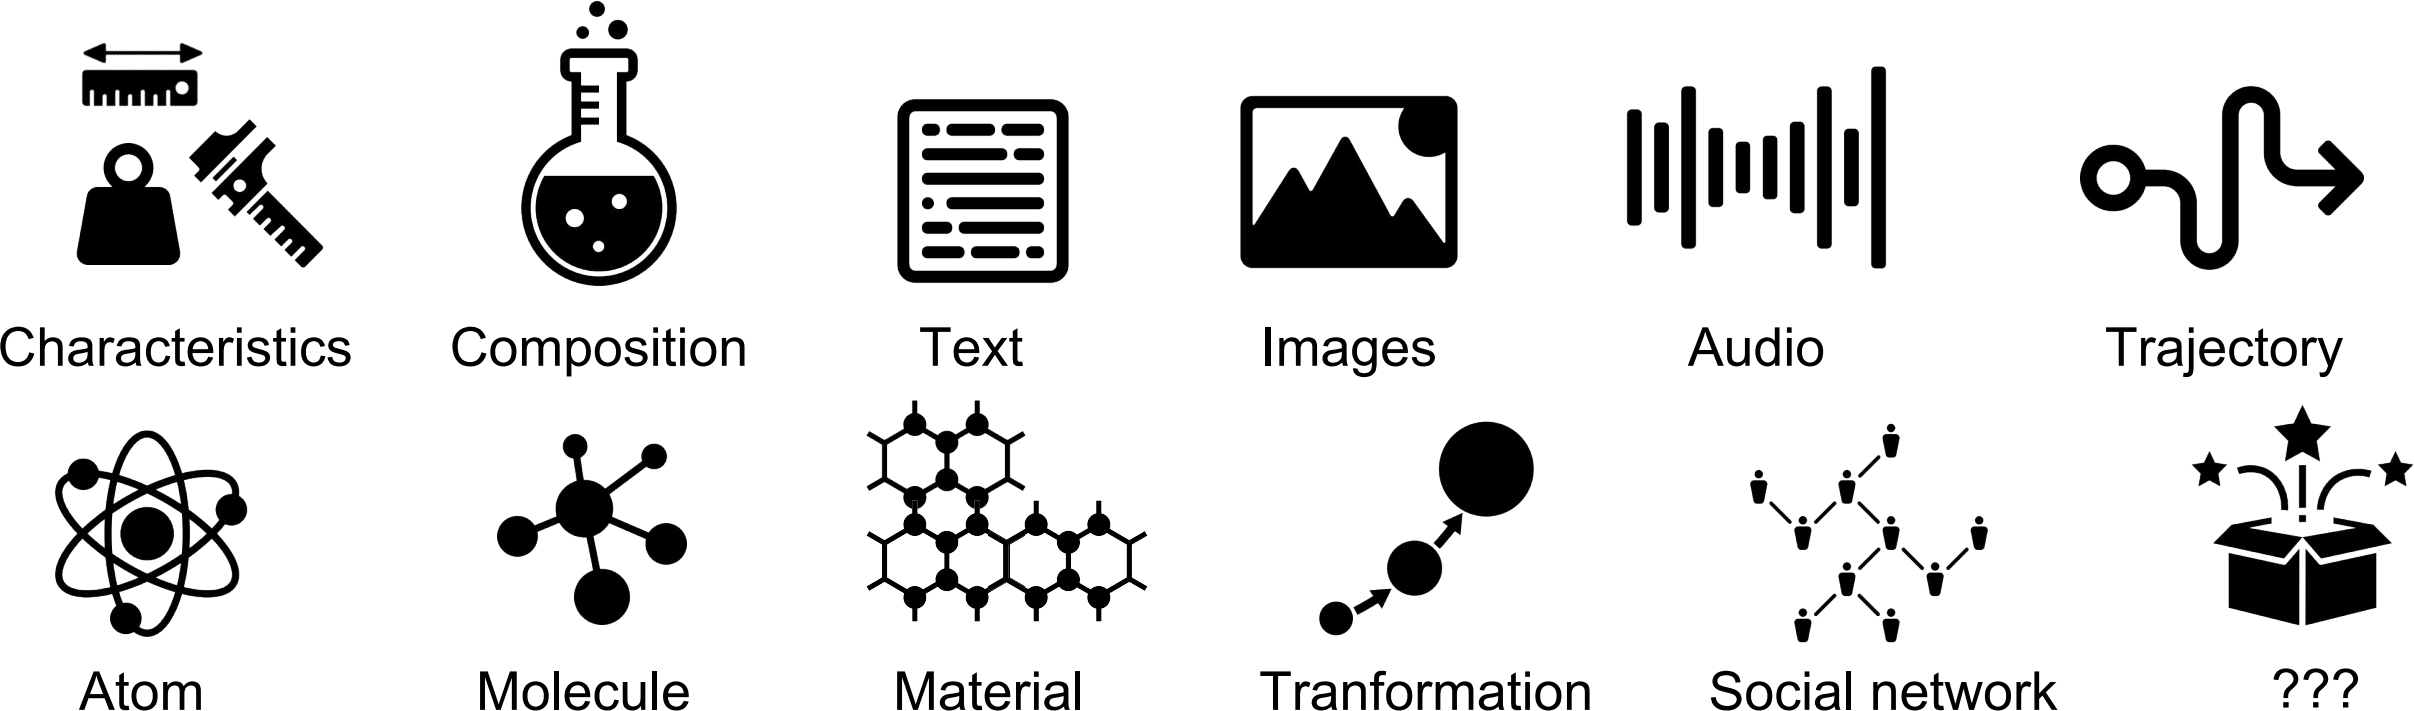
\includegraphics[width=\textwidth]{img/Data_Types.png}
    \end{center}
  \end{textblock}

  \begin{textblock}{90}(5, 60)
    \onslide<2->{
      To process them, we have to represent them numerically:
      \begin{itemize}
      \item Scalars, vectors, matrices, ...
      \item Time series
      \item Tokens
      \item Graphs
      \item Point clouds
      \item \etc{}
      \end{itemize}
    }
  \end{textblock}
\end{frame}


% Inspired by barra2006 (p. 7)
\begin{frame}
  \note{
    \begin{itemize}
    \item Big Data is not just a matter of size
    \item Give an overview of the 4V
    \item How would you rate GW data?
    \end{itemize}
  }
  \frametitle{Big data}

  \begin{block}{Not only size.}
    Data characterized by one or several V:
    \begin{itemize}
    \item<2-> \emph{Volume}: the volume of data is large
      \begin{itemize}
      \item TB, PB, EB,.. ?
      \item Big is when you can't handle the data on one computer
      \item How to process large amounts of data?
      \end{itemize}
    \item<3-> \emph{Velocity}: the growth rate of data is large
      \begin{itemize}
      \item 180h of new content every minute on Youtube
      \item How to cope with the rate of new data?
      \end{itemize}
    \item<4-> \emph{Variety}: the type and support of data is very different
      \begin{itemize}
      \item CSV files, images, videos, \etc{}
      \item Unstructured or semi-structured data
      \item How to find relations between those data?
      \end{itemize}
    \item<5-> \emph{Veracity}: data may not be reliable or truthful
      \begin{itemize}
      \item How to draw correct conclusions?
      \end{itemize}
    \item<6-> Other Vs?
    \end{itemize}
  \end{block}
\end{frame}


% Present the challenges of data
\begin{frame}
  \note{
    \begin{itemize}
    \item Provide some insights on data hell
    \item How would you rate GW data?
    \end{itemize}
  }
  \frametitle{Data hell}

  \begin{textblock}{90}(5, 15)
    \begin{block}{Obtaining good data is hard}
      \begin{itemize}
      \item<2-> Quantity:
        \begin{itemize}
        \item Too little: learning is hard
        \item Too much: technical difficulties
        \end{itemize}
      \item<3-> Representativity:
        \begin{itemize}
        \item Systematic biases
        \item Useless dimensions
        \end{itemize}
      \item<4-> Outliers, glitches
      \item<5-> Legal issues:
        \begin{itemize}
        \item GDPR
        \item Medical or other sensitive research
        \item Copyrights
        \item Confidentiality
        \end{itemize}
      \end{itemize}
      \onslide<6->{
        Data acquisition, cleaning and normalization can take up to 80\% of the
        time
      }
    \end{block}
  \end{textblock}
\end{frame}


% Present the important steps in a project
% Inspired by barra2006, chapter 2, section 1
\begin{frame}
  \frametitle{Steps in a \ac{ML} project}

  \begin{textblock}{90}(5, 15)
    \begin{enumerate}
      % 1.1.1 and 1.1.3
    \item Get familiar with the application domain and the type of data
      % 1.1.2
    \item Get the data and clarify input \& output of each step
      % 1.1.4
    \item Clean and normalize the data
      % 1.1.5
    \item Explore data:
      \begin{itemize}
      \item Descriptive statistics
      \item Visualization
      \end{itemize}
      % 1.1.7 (and 1.1.6)
    \item Compare various methods:
      \begin{itemize}
      \item Take into account the technical limits (computational power \&
        storage, \etc{})
      \item Establish a baseline (``classic method'') and compare other methods
        to it
      \end{itemize}
      % 1.1.8 and 1.1.9
    \item Optimimze and evaluate the method
    \item Deploy \& monitor the solution:
      \begin{itemize}
      \item Might require a different implementation to face run time constraints
      \end{itemize}
    \end{enumerate}
  \end{textblock}
\end{frame}


\subsection{Benefits, risks and challenges}

% Benefits/risks of ML
\begin{frame}
  \note{
    \begin{itemize}
    \item Present benefits and risks
    \item Almost each benefit as a potential counterpart
    \end{itemize}
  }
  \frametitle{Benefits and risks}

  \begin{textblock}{45}(5, 15)
    \begin{block}{Benefits}
      % Large scale deployment of \ac{ML} technology could benefit to:
      \begin{itemize}
      \item Deeper understanding of some phenomena:
        \begin{itemize}
        \item Prediction, classification, \etc{}
        \item Quantitative approach in Social Sciences
        \item Better modelling
        \end{itemize}
      \item Better services:
        \begin{itemize}
        \item Personalized medecine, smart cities, smart grids, \etc{}
        \item Personal assistant
        \end{itemize}
      \end{itemize}
    \end{block}
  \end{textblock}

  \begin{textblock}{45}(50, 15)
    \begin{block}{Risks}<2->
      % Large scale deployment of \ac{ML} technology could be detrimental to:
      \begin{itemize}
      \item Ethical aspects:
        \begin{itemize}
        \item Blind decision, discrimination
        \end{itemize}
      \item Legal aspects:
        \begin{itemize}
        \item Privacy, safety, security, copyrights
        \end{itemize}
      \item Cognitive effects:
        \begin{itemize}
        \item Loss of skills
        \item Attention span
        \end{itemize}
      \item Economical aspects:
        \begin{itemize}
        \item Disparition of jobs
        \item Over-importance of some companies
        \end{itemize}
      \item Environmental impact
      \end{itemize}
    \end{block}
  \end{textblock}
\end{frame}


% Challenges
% TODO: move in General Introduction?
\begin{frame}
  \frametitle{Challenges}

  \begin{textblock}{90}(5, 15)
    \begin{itemize}
    \item<1-> \acf{xAI}:
      \begin{itemize}
      \item Opening the black-box
      \item Interpretability: begin able to build indicators on the decision of the model
        (which variables are the most important, understand parts of the model)
      \item Explicability: being able to explain the decision of the model
      \end{itemize}
    \item<2-> Ethical \ac{AI}:
      \begin{itemize}
      \item Ethical guidelines regarding fundamental values, including such things as individual rights, privacy, non-discrimination, and non-manipulation
      \end{itemize}
    \item<3-> More technical challenges:
      \begin{itemize}
      \item Unsupervised learning
      \item New protocols: online learning, active learning
      \item Better understanding of data
      \end{itemize}
    \end{itemize}
  \end{textblock}
\end{frame}
